
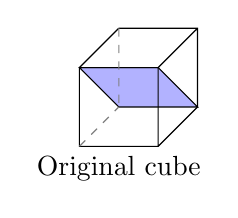
\begin{tikzpicture}
\filldraw[fill=blue!30!white, opacity=30,draw=black](0,1)--(1,1)--(1.5,0.5)--(0.5,0.5)--cycle;
\draw(0,0)rectangle(1,1)(1,1)--(1.5,1.5)(0,1)--(.5,1.5)(1,0)--(1.5,.5)(.5,1.5)--(1.5,1.5)--(1.5,0.5);
\draw[dashed, gray](0,0)--(0.5,0.5)(0.5,1.5)--(0.5,0.5);
\draw(0.5,0)node[anchor=north]{Original cube};
\end{tikzpicture}
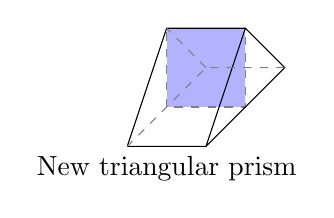
\begin{tikzpicture}
\filldraw[fill=blue!30!white,opacity=30,draw=gray, dashed](0,0)rectangle(1,1);
\draw(-0.5,-0.5)--(.5,-.5)--(1.5,.5)--(1,1)--(0.5,-0.5)(1,1)--(0,1)--(-.5,-.5);
\draw[gray, dashed](1.5,.5)--(0.5,0.5)--(-0.5,-0.5)(0.5,0.5)--(0,1);
\draw(0,-0.5)node[anchor=north]{New triangular prism};
\end{tikzpicture}

Note: Diagrams are \textbf{NOT} to scale.

A cube with side length $2$ is cut into two congruent triangular prisms.  The prisms are then reglued back together between two of their square faces.  What is the surface area of the new triangular prism formed in this process?



\ifsat
	\begin{enumerate}[label=\Alph*)]
		\item $12+4\sqrt{2} \approx 17.7$
		\item $24$
		\item $16+8\sqrt{2} \approx 27.3$%
		\item $32+16\sqrt{2} \approx 54.6$
	\end{enumerate}
\else
\fi

\ifacteven
	\begin{enumerate}[label=\textbf{\Alph*.},itemsep=\fill,align=left]
		\setcounter{enumii}{5}
		\item $8$
		\item $12+4\sqrt{2} \approx 17.7$
		\item $24$
		\addtocounter{enumii}{1}
		\item $16+8\sqrt{2} \approx 27.3$%
		\item $32+16\sqrt{2} \approx 54.6$
	\end{enumerate}
\else
\fi

\ifactodd
	\begin{enumerate}[label=\textbf{\Alph*.},itemsep=\fill,align=left]
		\item $8$
		\item $12+4\sqrt{2} \approx 17.7$
		\item $24$
		\item $16+8\sqrt{2} \approx 27.3$%
		\item $32+16\sqrt{2} \approx 54.6$
	\end{enumerate}
\else
\fi

\ifgridin
 $16+8\sqrt{2} \approx 27.3$%
		
\else
\fi

